\documentclass[aspectratio=169, 10pt]{beamer}

% ==============================================================================
% Packages
% ==============================================================================
\usepackage[utf8]{inputenc}
\usepackage[T1]{fontenc}
\usepackage{tgheros}
\renewcommand{\familydefault}{\sfdefault}
\usepackage{tikz}
\usetikzlibrary{shapes,arrows,positioning,calc,fit,backgrounds,decorations.pathreplacing}
\usepackage{graphicx}
\usepackage{booktabs}
\usepackage{tabularx}
\usepackage{colortbl}
\usepackage{xcolor}
\usepackage{hyperref}
\usepackage{array}

% ==============================================================================
% Color Definitions Matching Presentation
% ==============================================================================
\definecolor{themeblue}{RGB}{18, 0, 162}       % Right vertical accent bar & main theme
\definecolor{cardbg}{RGB}{241, 245, 254}        % Soft light-blue background for cards
\definecolor{cardborder}{RGB}{185, 208, 248}    % Card border
\definecolor{softblue}{RGB}{219, 234, 254}      % Light highlight blue
\definecolor{darkblue}{RGB}{12, 0, 120}        % Deep dark blue
\definecolor{bannerblue}{RGB}{18, 0, 162}      % Soft voting banner
\definecolor{chartblue}{RGB}{59, 130, 246}      % Bar chart vibrant blue
\definecolor{chartdarkblue}{RGB}{13, 71, 161}   % Dark bar blue
\definecolor{titlecolor}{RGB}{20, 20, 20}       % Headings
\definecolor{bodycolor}{RGB}{40, 40, 40}        % Text color
\definecolor{mutedgray}{RGB}{120, 120, 120}     % Axis & secondary text
\definecolor{linegray}{RGB}{228, 231, 236}      % Separator line

% ==============================================================================
% Hyperref & Citation Setup
% ==============================================================================
\hypersetup{
    colorlinks=true,
    linkcolor=themeblue,
    citecolor=themeblue,
    urlcolor=themeblue
}

% Ensure citations including brackets [1] are colored themeblue
\makeatletter
\def\@cite#1#2{\textcolor{themeblue}{[{#1\if@tempswa, #2\fi}]}}
\makeatother

% Clean Beamer Setup
\setbeamertemplate{navigation symbols}{}
\setbeamertemplate{bibliography item}[text]
\setbeamercolor{bibliography item}{fg=themeblue}
\setbeamercolor{bibliography entry author}{fg=bodycolor}
\setbeamercolor{bibliography entry title}{fg=bodycolor}
\setbeamercolor{bibliography entry location}{fg=bodycolor}
\setbeamercolor{bibliography entry note}{fg=bodycolor}
\setbeamertemplate{itemize item}{\small\textbullet}
\setbeamercolor{itemize item}{fg=black}
\setbeamersize{text margin left=0.8cm, text margin right=2.2cm}

% Background Canvas: Signature Right Accent Bar & Slide Numbering
\setbeamertemplate{background canvas}{%
  \begin{tikzpicture}[remember picture, overlay]
    % Right blue vertical stripe
    \fill[themeblue] ([xshift=-1.35cm]current page.north east) rectangle (current page.south east);
    % Slide number in white at bottom right
    \node[anchor=south, text=white, font=\large\bfseries] at ([xshift=-0.675cm, yshift=0.35cm]current page.south east) {\insertframenumber};
  \end{tikzpicture}%
}

% Frametitle formatting
\setbeamertemplate{frametitle}{%
  \vspace{0.35cm}%
  {\fontsize{18}{22}\selectfont\textbf{\color{titlecolor}\insertframetitle}}\par%
  \vspace{0.2cm}%
}

% Document Info
\title{VISUAL SPEECH RECOGNITION OF TAI PHAKE DIGITS}
\author{Champak Handique, Gargi Hatibaruah, Ishani Phukan, Milinda Barua}
\institute{Dibrugarh University Institute of Engineering and Technology}
\date{2026}

% ==============================================================================
% Document Body
% ==============================================================================
\begin{document}

% ------------------------------------------------------------------------------
% Slide 1: Title Slide
% ------------------------------------------------------------------------------
\begin{frame}
\vspace{-0.3cm}
\begin{center}
  % Dibrugarh University Seal Logo
  
\includegraphics[height=1.55cm]{figures/du_logo.png}\\[0.22cm]
  {\fontsize{10.5}{13.5}\selectfont\textbf{Dibrugarh University Institute of Engineering and Technology}}\\[0.1cm]
  {\fontsize{10}{13}\selectfont\textbf{FINAL YEAR PROJECT PROGRESS SEMINAR}}\\[0.55cm]
  {\fontsize{18}{23}\selectfont\textbf{VISUAL SPEECH RECOGNITION OF}}\\[0.1cm]
  {\fontsize{18}{23}\selectfont\textbf{TAI PHAKE DIGITS}}\\[0.65cm]
\end{center}

\vspace{0.25cm}
\noindent
\hspace{0.3cm}%
\begin{minipage}[t]{5.4cm}
  {\fontsize{9.5}{13}\selectfont
  \textbf{Group 8}\\[0.15cm]
  \begin{tabular}{@{}l@{\hspace{0.3cm}}l@{}}
    Sompu Handique & (CSE 23--14)\\
    Gargi Hatibaruah & (CSE 23--21)\\
    Ishani Phukan    & (CSE 23--27)\\
    Milinda Barua    & (CSE 23--41)
  \end{tabular}}
\end{minipage}%
\hspace{2.5cm}%
\begin{minipage}[t]{4.8cm}
  {\fontsize{9.5}{13}\selectfont
  \textbf{Under the Supervision of:}\\[0.15cm]
  Dr. Rabinder Kumar Prasad\\[0.06cm]
  Assistant Professor, DUIET}
\end{minipage}%
\end{frame}

% ------------------------------------------------------------------------------
% Slide 2: Contents
% ------------------------------------------------------------------------------
\begin{frame}
\frametitle{Contents}

\vspace{0.05cm}
\begin{columns}[onlytextwidth, T]
  \column{0.45\textwidth}
    \renewcommand{\arraystretch}{1.18}
    \begin{tabular}{@{}c@{\hspace{0.22cm}}l@{}}
      {\fontsize{13}{15}\selectfont\textbf{\color{themeblue}01}} & {\fontsize{9}{12}\selectfont Introduction} \\
      \multicolumn{2}{@{}l@{}}{\color{linegray}\rule{5.0cm}{0.4pt}} \\
      {\fontsize{13}{15}\selectfont\textbf{\color{themeblue}02}} & {\fontsize{9}{12}\selectfont Problem Statement} \\
      \multicolumn{2}{@{}l@{}}{\color{linegray}\rule{5.0cm}{0.4pt}} \\
      {\fontsize{13}{15}\selectfont\textbf{\color{themeblue}03}} & {\fontsize{9}{12}\selectfont Literature Review} \\
      \multicolumn{2}{@{}l@{}}{\color{linegray}\rule{5.0cm}{0.4pt}} \\
      {\fontsize{13}{15}\selectfont\textbf{\color{themeblue}04}} & {\fontsize{9}{12}\selectfont Flow diagram of our proposed work} \\
      \multicolumn{2}{@{}l@{}}{\color{linegray}\rule{5.0cm}{0.4pt}} \\
      {\fontsize{13}{15}\selectfont\textbf{\color{themeblue}05}} & {\fontsize{9}{12}\selectfont Preprocessing Pipeline} \\
      \multicolumn{2}{@{}l@{}}{\color{linegray}\rule{5.0cm}{0.4pt}} \\
      {\fontsize{13}{15}\selectfont\textbf{\color{themeblue}06}} & {\fontsize{9}{12}\selectfont Data Organization and class labels} \\
    \end{tabular}

  \column{0.54\textwidth}
    \renewcommand{\arraystretch}{1.18}
    \begin{tabular}{@{}c@{\hspace{0.22cm}}l@{}}
      {\fontsize{13}{15}\selectfont\textbf{\color{themeblue}07}} & {\fontsize{9}{12}\selectfont Results till date} \\
      \multicolumn{2}{@{}l@{}}{\color{linegray}\rule{5.4cm}{0.4pt}} \\
      {\fontsize{13}{15}\selectfont\textbf{\color{themeblue}08}} & {\fontsize{9}{12}\selectfont Three Model Ensemble} \\
      \multicolumn{2}{@{}l@{}}{\color{linegray}\rule{5.4cm}{0.4pt}} \\
      {\fontsize{13}{15}\selectfont\textbf{\color{themeblue}09}} & {\fontsize{9}{12}\selectfont Error Analysis and Targetted Improvements} \\
      \multicolumn{2}{@{}l@{}}{\color{linegray}\rule{5.4cm}{0.4pt}} \\
      {\fontsize{13}{15}\selectfont\textbf{\color{themeblue}10}} & {\fontsize{9}{12}\selectfont Conclusion, Limitations and Next Steps} \\
      \multicolumn{2}{@{}l@{}}{\color{linegray}\rule{5.4cm}{0.4pt}} \\
      {\fontsize{13}{15}\selectfont\textbf{\color{themeblue}11}} & {\fontsize{9}{12}\selectfont References} \\
    \end{tabular}
\end{columns}
\end{frame}

% ------------------------------------------------------------------------------
% Slide 3: Introduction
% ------------------------------------------------------------------------------
\begin{frame}
\frametitle{Introduction}

\begin{columns}[onlytextwidth, T]
  \column{0.60\textwidth}
    {\fontsize{13}{16}\selectfont\textbf{\color{themeblue}Visual Speech Recognition}}\\[0.2cm]
    {\fontsize{10}{14}\selectfont
    Visual Speech Recognition (VSR), also called lip reading, predicts spoken content from visible mouth movements in video. It is useful when audio is unavailable or unreliable\cite{chung2017}.}\\[0.65cm]

    {\fontsize{13}{16}\selectfont\textbf{\color{themeblue}Why Tai Phake?}}\\[0.2cm]
    {\fontsize{10}{14}\selectfont
    The project uses Visual Speech Recognition (VSR) to recognise Tai Phake, a language with no lip reading research and limited resources\cite{kim2023}\cite{yeo2023}. It focuses on identifying 11 classes from silent video clips.}

  \column{0.38\textwidth}
    \begin{center}
    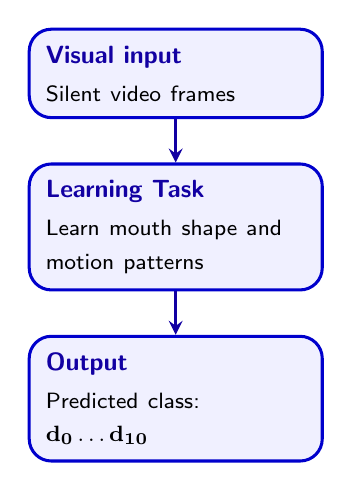
\begin{tikzpicture}[
      box/.style={
        draw=blue!80!black,
        line width=1.1pt,
        fill=blue!6,
        rounded corners=8pt,
        text width=3.3cm,
        inner sep=6pt,
        align=left
      },
      arrow/.style={->, >=stealth, line width=1.2pt, color=themeblue}
    ]
      % Box 1: Visual input
      \node[box] (b1) at (0, 0) {
        {\fontsize{9.5}{12}\selectfont\textbf{\color{themeblue}Visual input}}\\[0.06cm]
        {\fontsize{8.5}{11}\selectfont Silent video frames}
      };

      % Box 2: Learning Task
      \node[box, below=0.55cm of b1] (b2) {
        {\fontsize{9.5}{12}\selectfont\textbf{\color{themeblue}Learning Task}}\\[0.06cm]
        {\fontsize{8.5}{11}\selectfont Learn mouth shape and motion patterns}
      };

      % Box 3: Output
      \node[box, below=0.55cm of b2] (b3) {
        {\fontsize{9.5}{12}\selectfont\textbf{\color{themeblue}Output}}\\[0.06cm]
        {\fontsize{8.5}{11}\selectfont Predicted class: $\mathbf{d_0 \dots d_{10}}$}
      };

      % Connectors
      \draw[arrow] (b1.south) -- (b2.north);
      \draw[arrow] (b2.south) -- (b3.north);
    \end{tikzpicture}
    \end{center}
\end{columns}
\end{frame}

% ------------------------------------------------------------------------------
% Slide 4: Problem Statement
% ------------------------------------------------------------------------------
\begin{frame}
\frametitle{Problem Statement}

\vspace{0.1cm}
{\fontsize{10.5}{15.5}\selectfont
Tai Phake is a low resource language spoken by approximately 1,400 to 2,000 people\cite{deka2025}, primarily in Assam and Arunachal Pradesh in Northeast India. The small number of speakers makes it challenging to collect sufficient data for language technology research.\\[0.45cm]

Lip-reading research for Tai Phake is limited. Related work exists for neighbouring languages, e.g. Assamese\cite{prasad2025}, and Khasi\cite{lyngdoh2026}. Recognizing spoken digits from lip movements alone is difficult because mouth movements vary across speakers\cite{lyngdoh2026}.\\[0.45cm]

In this project, we develop and compare deep learning models, including CNN--RNN, pretrained CNN, Transformer, attention-based, and motion-based models\cite{prasad2025},\cite{prajwal2022},\cite{chung2017}. Our goal is to identify an effective approach for recognizing Tai Phake digits from video clips without using audio.}
\end{frame}

% ------------------------------------------------------------------------------
% Slide 5: Literature Review (Part 1)
% ------------------------------------------------------------------------------
\begin{frame}
\frametitle{Literature Review}

\vspace{-0.1cm}
\begin{center}
\renewcommand{\arraystretch}{1.22}
\setlength{\tabcolsep}{3.5pt}
{\fontsize{6.8}{8.8}\selectfont
\begin{tabular}{|>{\centering\arraybackslash}m{2.05cm}|>{\centering\arraybackslash}m{2.35cm}|>{\centering\arraybackslash}m{2.0cm}|>{\centering\arraybackslash}m{1.8cm}|>{\centering\arraybackslash}m{3.45cm}|}
  \hline
  \textbf{Paper} & \textbf{Method} & \textbf{Dataset} & \begin{tabular}[c]{@{}c@{}}\textbf{Reported}\\\textbf{Performance}\end{tabular} & \textbf{Limitation} \\
  \hline
  \begin{tabular}[c]{@{}c@{}}\textbf{\cite{prasad2025}} Prasad et al.\\ (2025)\end{tabular} & 2D/3D CNN + LSTM/GRU & Assamese Digit Dataset ($d_0$--$d_9$) & 83\% (CNN--LSTM) & Small speaker sample; sensitive to lighting and speaker variation \\
  \hline
  \begin{tabular}[c]{@{}c@{}}\textbf{\cite{lyngdoh2026}} Lyngdoh \&\\ Maji (2026)\end{tabular} & Feature extraction + traditional ML classifiers & Khasi language corpus & 94.44\% (SVM), 80.86\% (KNN) & Limited deep spatiotemporal modeling; performance drops on unseen speakers \\
  \hline
  \begin{tabular}[c]{@{}c@{}}\textbf{\cite{kim2023}} Kim et al.\\ (2023)\end{tabular} & Cross-lingual pretraining + language-specific classifier heads & LRW/LRS2; low-resource multilingual datasets & WER varies by language & Requires a large high-resource pretraining dataset; viseme collisions remain challenging \\
  \hline
  \begin{tabular}[c]{@{}c@{}}\textbf{\cite{yeo2023}} Yeo et al.\\ (2023)\end{tabular} & Whisper-based pseudo-labeling & Multilingual video and speech data & WER varies by language & Depends on Whisper supporting the target language \\
  \hline
\end{tabular}}
\end{center}
\end{frame}

% ------------------------------------------------------------------------------
% Slide 6: Literature Review (Part 2)
% ------------------------------------------------------------------------------
\begin{frame}
\frametitle{Literature Review}

\vspace{-0.1cm}
\begin{center}
\renewcommand{\arraystretch}{1.22}
\setlength{\tabcolsep}{3.5pt}
{\fontsize{6.8}{8.8}\selectfont
\begin{tabular}{|>{\centering\arraybackslash}m{2.05cm}|>{\centering\arraybackslash}m{2.35cm}|>{\centering\arraybackslash}m{2.0cm}|>{\centering\arraybackslash}m{1.8cm}|>{\centering\arraybackslash}m{3.45cm}|}
  \hline
  \textbf{Paper} & \textbf{Method} & \textbf{Dataset} & \begin{tabular}[c]{@{}c@{}}\textbf{Reported}\\\textbf{Performance}\end{tabular} & \textbf{Limitation} \\
  \hline
  \begin{tabular}[c]{@{}c@{}}\textbf{\cite{prajwal2022}} Prajwal et al.\\ (2022)\end{tabular} & Multi-scale spatiotemporal visual attention & LRW and LRS3 & \begin{tabular}[c]{@{}c@{}}22.6\% WER\\ LRS2\end{tabular} & High computational complexity; requires substantial training data \\
  \hline
  \begin{tabular}[c]{@{}c@{}}\textbf{\cite{chung2017}} Chung \&\\ Zisserman (2017)\end{tabular} & 2D/3D CNN + LSTM & LRW (500 English words) & & Requires extensive training data; focuses on English broadcast videos \\
  \hline
  \begin{tabular}[c]{@{}c@{}}\textbf{\cite{rahmatullah2025}} Rahmatullah\\ et al.\ (2025)\end{tabular} & Attention-enhanced ResNet + recurrent-transformer encoder & Low-resource VSR benchmarks & & Complex training pipeline; curriculum learning requires tuning \\
  \hline
  \begin{tabular}[c]{@{}c@{}}\textbf{\cite{thomas2025}} Thomas et al.\\ (2025)\end{tabular} & VALLR: visual encoder + LLM decoder & LRS2 and LRS3 & \begin{tabular}[c]{@{}c@{}}18.7\% (LRS3),\\ 20.8\% (LRS2)\end{tabular} & High computational and parameter requirements; unsuitable for extremely low-resource languages \\
  \hline
\end{tabular}}
\end{center}
\end{frame}

% ------------------------------------------------------------------------------
% Slide 7: Flow diagram of our proposed work
% ------------------------------------------------------------------------------
\begin{frame}
\frametitle{Flow diagram of our proposed work}

\vspace{-0.1cm}
\begin{center}
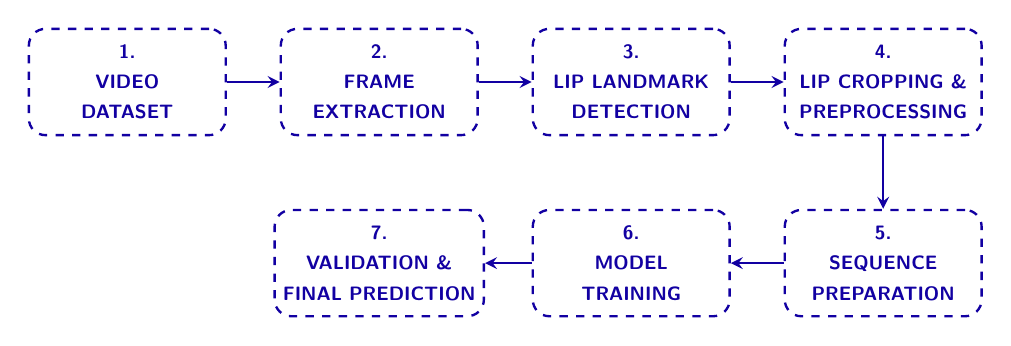
\begin{tikzpicture}[
  flownode/.style={
    draw=themeblue,
    dashed,
    line width=0.85pt,
    rounded corners=6pt,
    fill=white,
    minimum width=2.5cm,
    minimum height=1.35cm,
    align=center,
    font=\fontsize{7.5}{9.5}\selectfont\bfseries\color{themeblue},
    inner sep=3pt
  },
  flowarrow/.style={
    ->,
    >=stealth,
    line width=0.9pt,
    themeblue
  }
]
  % Row 1: 1 -> 2 -> 3 -> 4
  \node[flownode] (f1) at (0, 0)     {1.\\[0.05cm]VIDEO\\[0.05cm]DATASET};
  \node[flownode] (f2) at (3.2, 0)   {2.\\[0.05cm]FRAME\\[0.05cm]EXTRACTION};
  \node[flownode] (f3) at (6.4, 0)   {3.\\[0.05cm]LIP LANDMARK\\[0.05cm]DETECTION};
  \node[flownode] (f4) at (9.6, 0)   {4.\\[0.05cm]LIP CROPPING \&\\[0.05cm]PREPROCESSING};

  % Row 2: 7 <- 6 <- 5
  \node[flownode] (f5) at (9.6, -2.3) {5.\\[0.05cm]SEQUENCE\\[0.05cm]PREPARATION};
  \node[flownode] (f6) at (6.4, -2.3) {6.\\[0.05cm]MODEL\\[0.05cm]TRAINING};
  \node[flownode] (f7) at (3.2, -2.3) {7.\\[0.05cm]VALIDATION \&\\[0.05cm]FINAL PREDICTION};

  % Connecting Arrows
  \draw[flowarrow] (f1) -- (f2);
  \draw[flowarrow] (f2) -- (f3);
  \draw[flowarrow] (f3) -- (f4);
  \draw[flowarrow] (f4) -- (f5);
  \draw[flowarrow] (f5) -- (f6);
  \draw[flowarrow] (f6) -- (f7);
\end{tikzpicture}
\end{center}
\end{frame}

% ------------------------------------------------------------------------------
% Slide 8: Preprocessing Pipeline
% ------------------------------------------------------------------------------
\begin{frame}
\frametitle{Preprocessing Pipeline}

\vspace{-0.55cm}
% Top horizontal pipeline (1 to 5)
\begin{center}
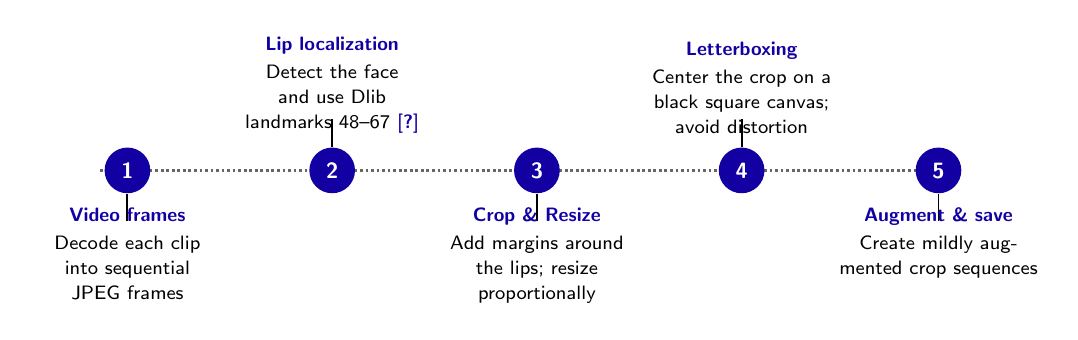
\begin{tikzpicture}[
  pipenode/.style={
    circle,
    fill=themeblue,
    text=white,
    font=\fontsize{8.5}{10}\selectfont\bfseries,
    inner sep=3pt,
    minimum size=0.58cm
  }
]
  % Dotted connecting line
  \draw[densely dotted, color=black!60, line width=1.0pt] (0, 0) -- (10.9, 0);

  % 1: Video frames
  \node[pipenode] (p1) at (0.35, 0) {1};
  \draw[line width=0.7pt] (p1.south) -- ++(0, -0.35);
  \node[align=center, anchor=north, text width=2.3cm, font=\fontsize{7}{9}\selectfont] at (0.35, -0.35) {
    \textbf{\color{themeblue}Video frames}\\[0.04cm]
    Decode each clip into sequential JPEG frames
  };

  % 2: Lip localization
  \node[pipenode] (p2) at (2.95, 0) {2};
  \draw[line width=0.7pt] (p2.north) -- ++(0, 0.35);
  \node[align=center, anchor=south, text width=2.4cm, font=\fontsize{7}{9}\selectfont] at (2.95, 0.35) {
    \textbf{\color{themeblue}Lip localization}\\[0.04cm]
    Detect the face and use Dlib landmarks 48--67~\cite{prasad2025}
  };

  % 3: Crop & Resize
  \node[pipenode] (p3) at (5.55, 0) {3};
  \draw[line width=0.7pt] (p3.south) -- ++(0, -0.35);
  \node[align=center, anchor=north, text width=2.5cm, font=\fontsize{7}{9}\selectfont] at (5.55, -0.35) {
    \textbf{\color{themeblue}Crop \& Resize}\\[0.04cm]
    Add margins around the lips; resize proportionally
  };

  % 4: Letterboxing
  \node[pipenode] (p4) at (8.15, 0) {4};
  \draw[line width=0.7pt] (p4.north) -- ++(0, 0.35);
  \node[align=center, anchor=south, text width=2.6cm, font=\fontsize{7}{9}\selectfont] at (8.15, 0.35) {
    \textbf{\color{themeblue}Letterboxing}\\[0.04cm]
    Center the crop on a black square canvas; avoid distortion
  };

  % 5: Augment & save
  \node[pipenode] (p5) at (10.65, 0) {5};
  \draw[line width=0.7pt] (p5.south) -- ++(0, -0.35);
  \node[align=center, anchor=north, text width=2.6cm, font=\fontsize{7}{9}\selectfont] at (10.65, -0.35) {
    \textbf{\color{themeblue}Augment \& save}\\[0.04cm]
    Create mildly augmented crop sequences
  };
\end{tikzpicture}
\end{center}

\vspace{0.12cm}%
% Bottom two cards
\noindent
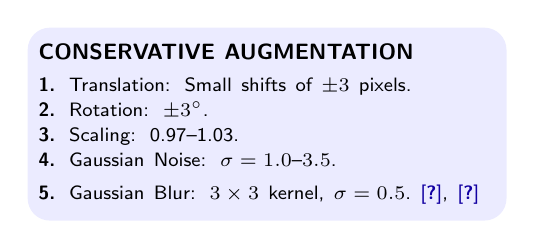
\begin{tikzpicture}
  \node[draw=none, fill=blue!8, rounded corners=8pt, text width=5.8cm, inner sep=4pt, minimum height=2.45cm] {
    {\fontsize{8.5}{10.5}\selectfont\textbf{CONSERVATIVE AUGMENTATION}}\\[0.1cm]
    {\fontsize{7}{9}\selectfont
    \textbf{1.} Translation: Small shifts of $\pm 3$ pixels.\\
    \textbf{2.} Rotation: $\pm 3^\circ$.\\
    \textbf{3.} Scaling: 0.97--1.03.\\
    \textbf{4.} Gaussian Noise: $\sigma = 1.0$--$3.5$.\\
    \textbf{5.} Gaussian Blur: $3 \times 3$ kernel, $\sigma = 0.5$.~\cite{prasad2025}, \cite{prajwal2022}}
  };
\end{tikzpicture}%
\hfill
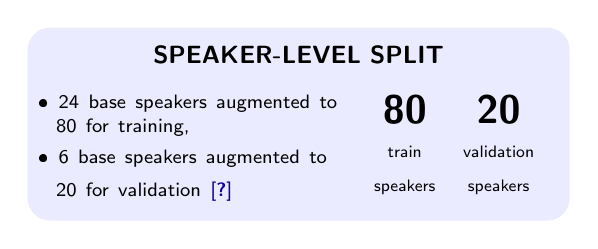
\begin{tikzpicture}
  \node[draw=none, fill=blue!8, rounded corners=8pt, text width=6.6cm, inner sep=4pt, minimum height=2.45cm] {
    {\centering {\fontsize{9.5}{12}\selectfont\textbf{SPEAKER-LEVEL SPLIT}}\par}
    \vspace{0.36cm}
    \begin{minipage}[c]{3.85cm}
      \raggedright
      {\fontsize{6.8}{8.8}\selectfont
      \textbullet~24 base speakers augmented to\\
      \hspace*{0.22cm}80 for training,\\[0.08cm]
      \textbullet~6 base speakers augmented to\\
      \hspace*{0.22cm}20 for validation~\cite{lyngdoh2026}}
    \end{minipage}%
    \hfill
    \begin{minipage}[c]{2.65cm}
      \centering
      \begin{tabular}{@{}c@{\hspace{0.35cm}}c@{}}
        {\fontsize{15}{17}\selectfont\textbf{80}} & {\fontsize{15}{17}\selectfont\textbf{20}} \\[0.02cm]
        {\fontsize{6.5}{8}\selectfont train} & {\fontsize{6.5}{8}\selectfont validation} \\
        {\fontsize{6.5}{8}\selectfont speakers} & {\fontsize{6.5}{8}\selectfont speakers}
      \end{tabular}
    \end{minipage}
  };
\end{tikzpicture}
\end{frame}

% ------------------------------------------------------------------------------
% Slide 9: Data organisation and class labels
% ------------------------------------------------------------------------------
\begin{frame}
\frametitle{Data organisation and class labels}

\begin{columns}[onlytextwidth, c]
  \column{0.48\textwidth}
    {\fontsize{12}{15}\selectfont\textbf{\color{themeblue}$\bullet$ 330 Original Video Clips}}\\[0.1cm]
    {\fontsize{9}{12.5}\selectfont 30 speakers $\times$ 11 clips~\cite{prasad2025} .mp4 source\\
    videos (one spoken digit per clip)}\\[0.35cm]

    {\fontsize{12}{15}\selectfont\textbf{\color{themeblue}$\bullet$ 96 X 96 RGB lip crops}}\\[0.1cm]
    {\fontsize{9}{12.5}\selectfont $\sim$30 sampled frames per clip (region of interest)}\\[0.35cm]

    {\fontsize{12}{15}\selectfont\textbf{\color{themeblue}$\bullet$ 11 Class Labels}}\\[0.1cm]
    {\fontsize{9}{12.5}\selectfont 11 labels, d0 to d10: \textbf{pao, naung, song, saam, s\={i}, ha\={a}, howk, cheit, peat, kao, sip}}

  \column{0.50\textwidth}
    \begin{center}
      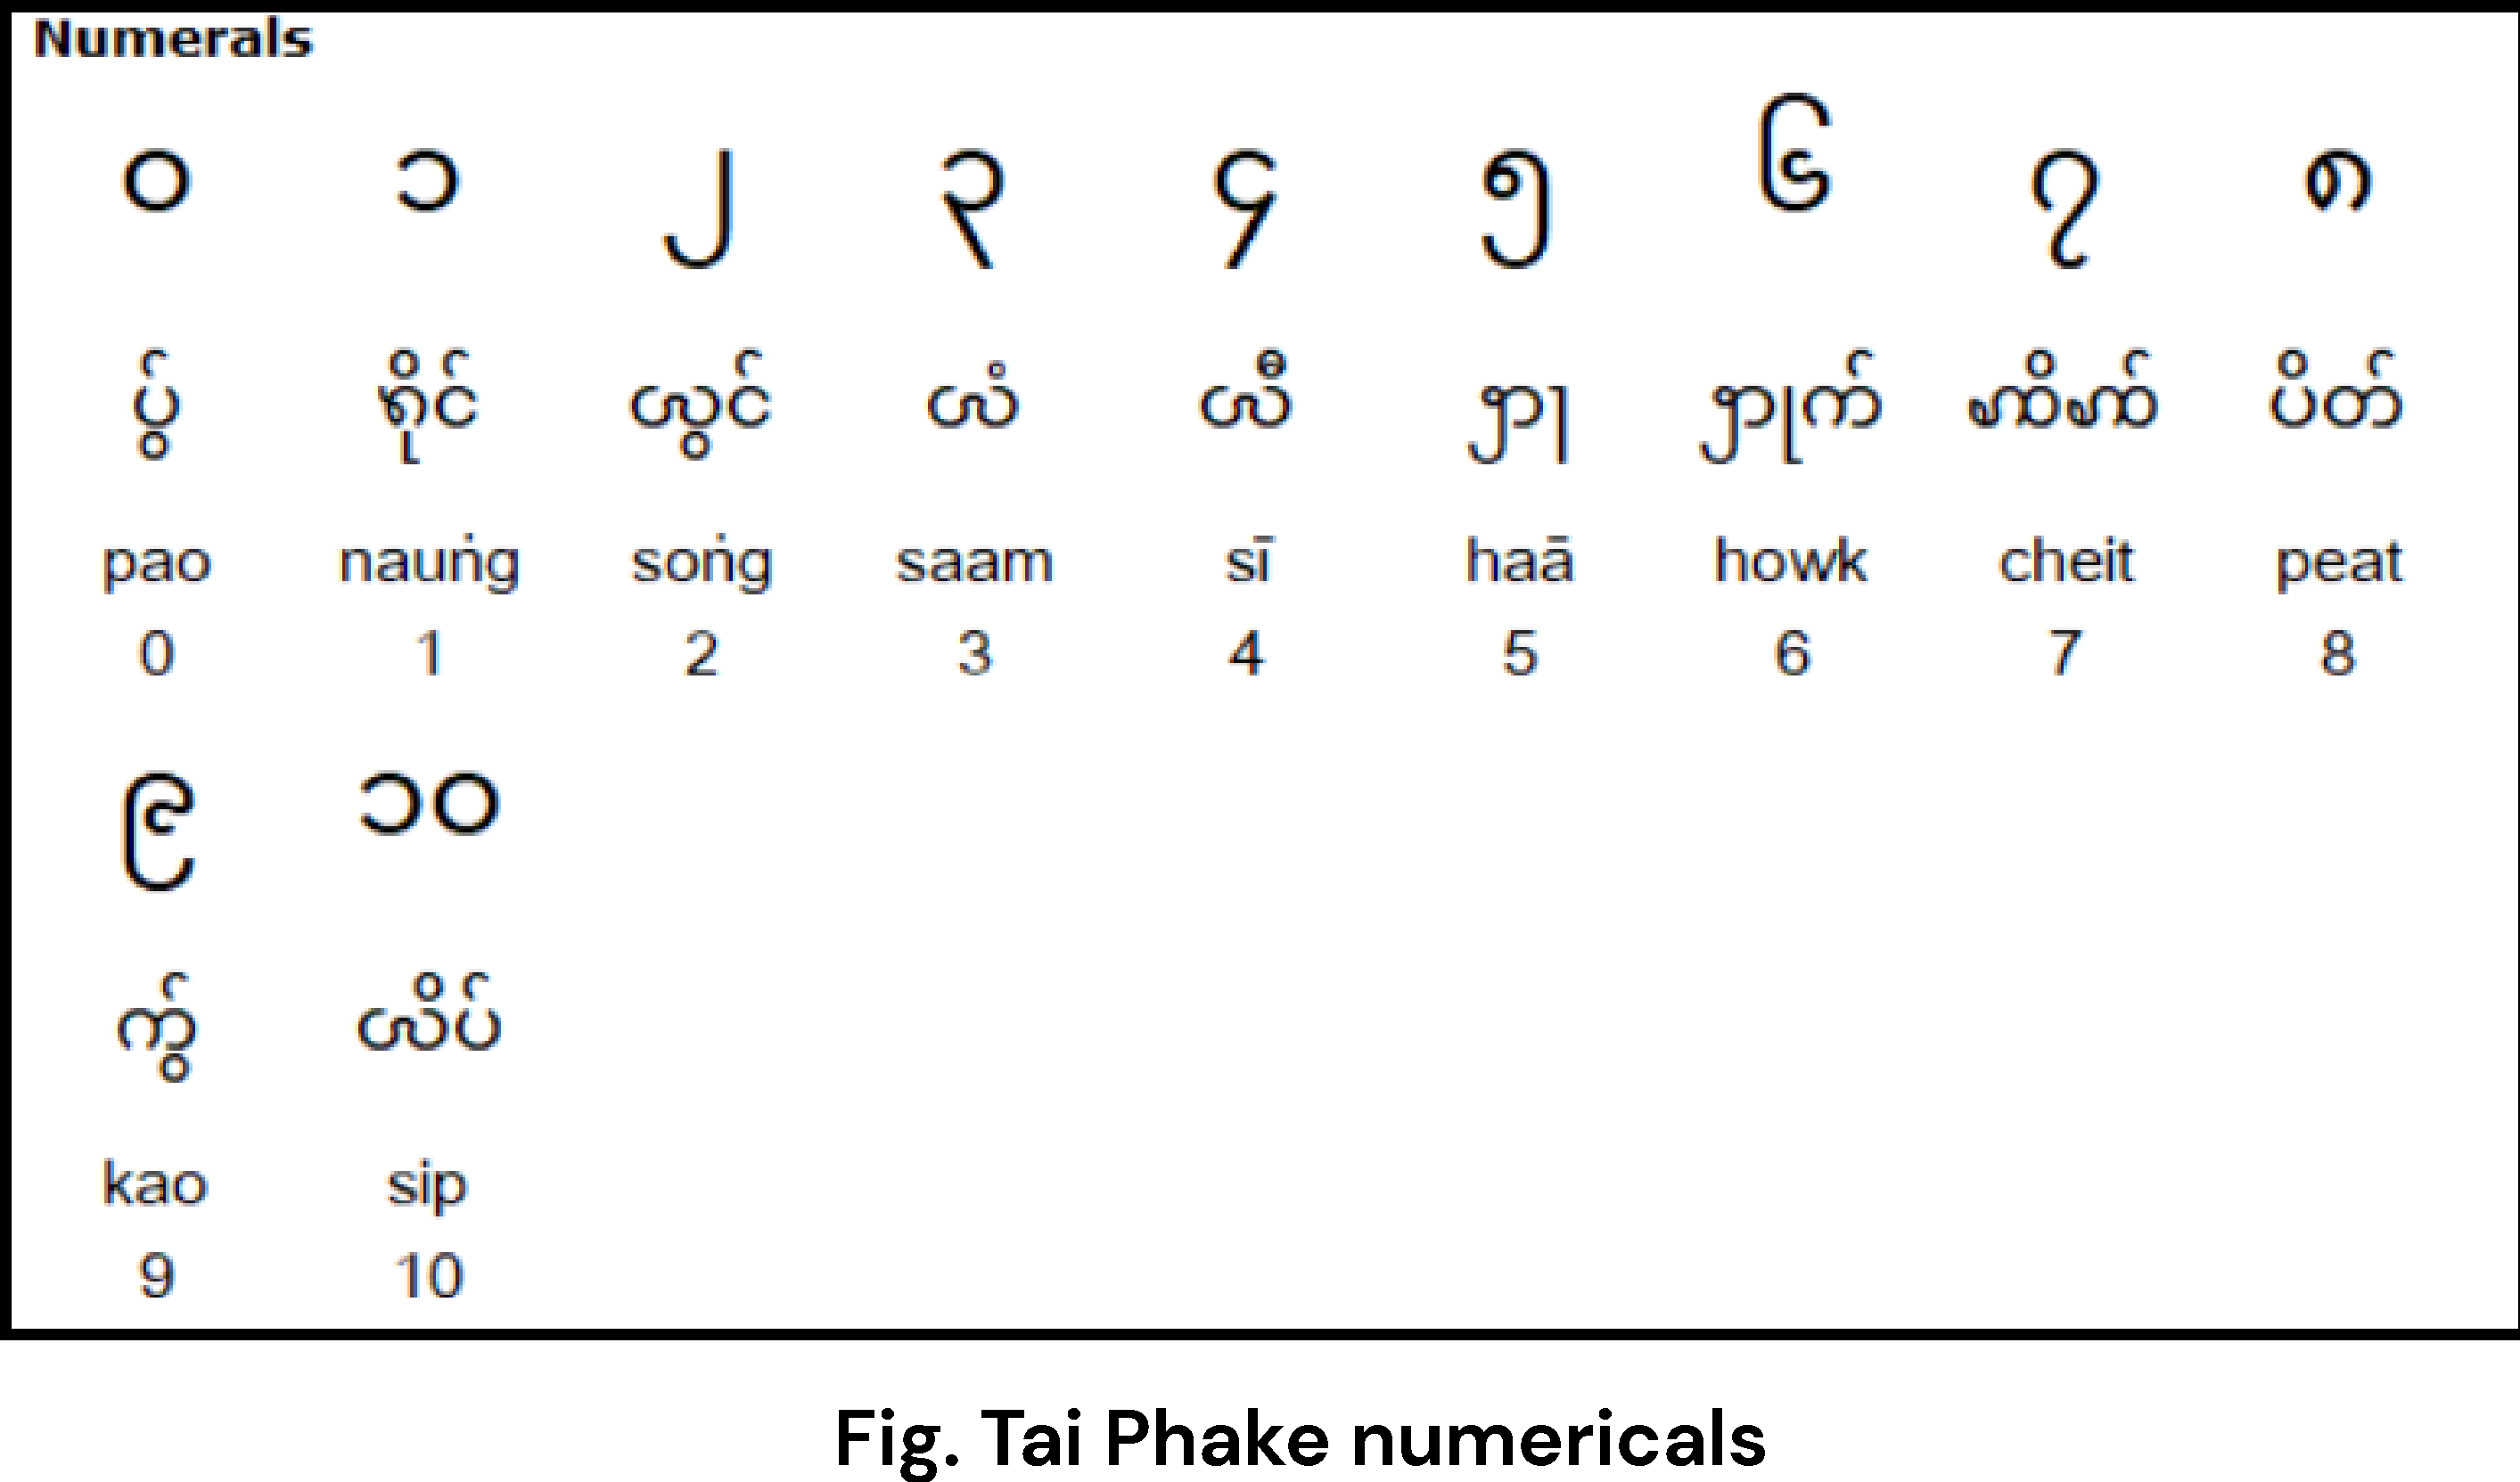
\includegraphics[width=0.92\linewidth]{figures/tai_phake_numerals_box.png}
    \end{center}
\end{columns}
\end{frame}

% ------------------------------------------------------------------------------
% Slide 10: Results till date
% ------------------------------------------------------------------------------
\begin{frame}
\frametitle{Results till date}

\vspace{-0.2cm}
{\fontsize{10.5}{13}\selectfont\textbf{Reported Validation Accuracy}}\\[0.25cm]

\begin{columns}[onlytextwidth, c]
  \column{0.47\textwidth}
    \renewcommand{\arraystretch}{1.25}
    {\fontsize{7.5}{9.5}\selectfont
    \begin{tabular}{|>{\raggedright\arraybackslash}p{2.6cm}|c|}
      \hline
      \rowcolor{blue!15}
      \textbf{Experimental Phase} & \parbox{2.0cm}{\centering\textbf{Reported}\\[-0.03cm]\textbf{Accuracy}} \\
      \hline
      Chance Reference & 9.09\% \\
      \hline
      MobileNetV2 Transfer Learning & 57.58\% \\
      \hline
      Class Weighing & 71.36\% \\
      \hline
      Two model Ensemble & 76.82\% \\
      \hline
      \textbf{Three model Ensemble} & \textbf{81.36\%} \\
      & {\fontsize{6.5}{8}\selectfont Macro F1 score: 0.8137} \\
      \hline
    \end{tabular}}

  \column{0.51\textwidth}
    \begin{center}
    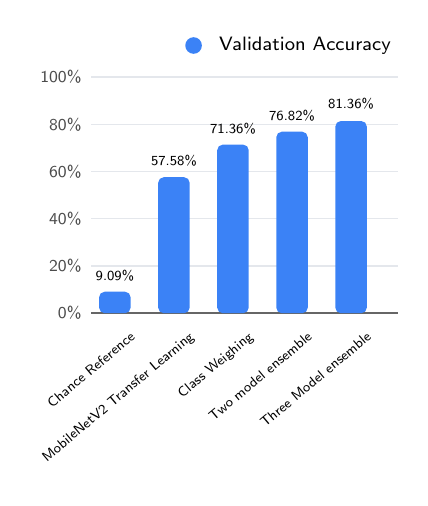
\begin{tikzpicture}[font=\fontsize{6.5}{8}\selectfont]
      % Legend
      \fill[chartblue] (1.3, 3.4) circle (3pt);
      \node[right, font=\fontsize{7}{9}\selectfont] at (1.5, 3.4) {Validation Accuracy};

      % Y-axis ticks and horizontal grid lines
      \foreach \y/\label in {0/0\%, 0.6/20\%, 1.2/40\%, 1.8/60\%, 2.4/80\%, 3.0/100\%} {
        \draw[linegray, line width=0.4pt] (0, \y) -- (3.9, \y);
        \node[left, text=black!70] at (0, \y) {\label};
      }
      \draw[black!60, line width=0.6pt] (0, 0) -- (3.9, 0);

      % Bar 1: Chance Reference: 9.09% -> (9.09/100)*3.0 = 0.273 cm
      \fill[chartblue, rounded corners=2pt] (0.1, 0) rectangle (0.5, 0.273);
      \node[anchor=south, font=\fontsize{5.5}{7}\selectfont] at (0.3, 0.28) {9.09\%};
      \node[anchor=north east, rotate=40, font=\fontsize{5.5}{7}\selectfont] at (0.5, -0.05) {Chance Reference};

      % Bar 2: MobileNetV2 Transfer: 57.58% -> 1.727 cm
      \fill[chartblue, rounded corners=2pt] (0.85, 0) rectangle (1.25, 1.727);
      \node[anchor=south, font=\fontsize{5.5}{7}\selectfont] at (1.05, 1.74) {57.58\%};
      \node[anchor=north east, rotate=40, font=\fontsize{5.5}{7}\selectfont] at (1.25, -0.05) {MobileNetV2 Transfer Learning};

      % Bar 3: Class Weighing: 71.36% -> 2.141 cm
      \fill[chartblue, rounded corners=2pt] (1.6, 0) rectangle (2.0, 2.141);
      \node[anchor=south, font=\fontsize{5.5}{7}\selectfont] at (1.8, 2.15) {71.36\%};
      \node[anchor=north east, rotate=40, font=\fontsize{5.5}{7}\selectfont] at (2.0, -0.05) {Class Weighing};

      % Bar 4: Two model ensemble: 76.82% -> 2.305 cm
      \fill[chartblue, rounded corners=2pt] (2.35, 0) rectangle (2.75, 2.305);
      \node[anchor=south, font=\fontsize{5.5}{7}\selectfont] at (2.55, 2.32) {76.82\%};
      \node[anchor=north east, rotate=40, font=\fontsize{5.5}{7}\selectfont] at (2.75, -0.05) {Two model ensemble};

      % Bar 5: Three Model ensemble: 81.36% -> 2.441 cm
      \fill[chartblue, rounded corners=2pt] (3.1, 0) rectangle (3.5, 2.441);
      \node[anchor=south, font=\fontsize{5.5}{7}\selectfont] at (3.3, 2.46) {81.36\%};
      \node[anchor=north east, rotate=40, font=\fontsize{5.5}{7}\selectfont] at (3.5, -0.05) {Three Model ensemble};
    \end{tikzpicture}
    \end{center}
\end{columns}
\end{frame}

% ------------------------------------------------------------------------------
% Slide 11: Three model ensemble: 81.36%
% ------------------------------------------------------------------------------
\begin{frame}
\frametitle{Three model\\[-0.05cm]ensemble: 81.36\%}

\begin{columns}[onlytextwidth, c]
  \column{0.51\textwidth}
    \renewcommand{\arraystretch}{1.18}
    {\fontsize{7}{9}\selectfont
    \begin{tabular}{|>{\raggedright\arraybackslash}p{2.6cm}|c|c|}
      \hline
      \rowcolor{darkblue}
      \textbf{\color{white}Model} & \textbf{\color{white}Weight} & \parbox{1.8cm}{\centering\textbf{\color{white}Validation}\\[-0.03cm]\textbf{\color{white}Accuracy}} \\
      \hline
      A: EfficientNetB0 + motion + BiGRU & 0.15 & 70.45\% \\
      \hline
      B: MobileNetV2 + BiLSTM + attention & 0.4 & 68.18\% \\
      \hline
      C: EffNet-B0 + tri-window+neutraliser & 0.45 & 69.09\% \\
      \hline
      \rowcolor{blue!15}
      \textbf{Fusion with 4-view TTA per model} & & \textbf{81.36\%} \\
      \hline
    \end{tabular}}

    \vspace{0.45cm}
    \begin{center}
    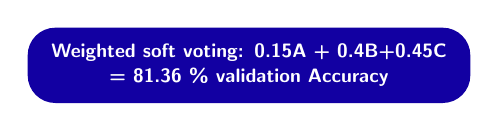
\begin{tikzpicture}
      \node[draw=none, fill=themeblue, rounded corners=10pt, text=white, font=\fontsize{7}{9}\selectfont\bfseries, inner sep=6pt, text width=5.2cm, align=center] {
        Weighted soft voting: 0.15A + 0.4B+0.45C = 81.36 \% validation Accuracy
      };
    \end{tikzpicture}
    \end{center}

  \column{0.47\textwidth}
    \begin{center}
      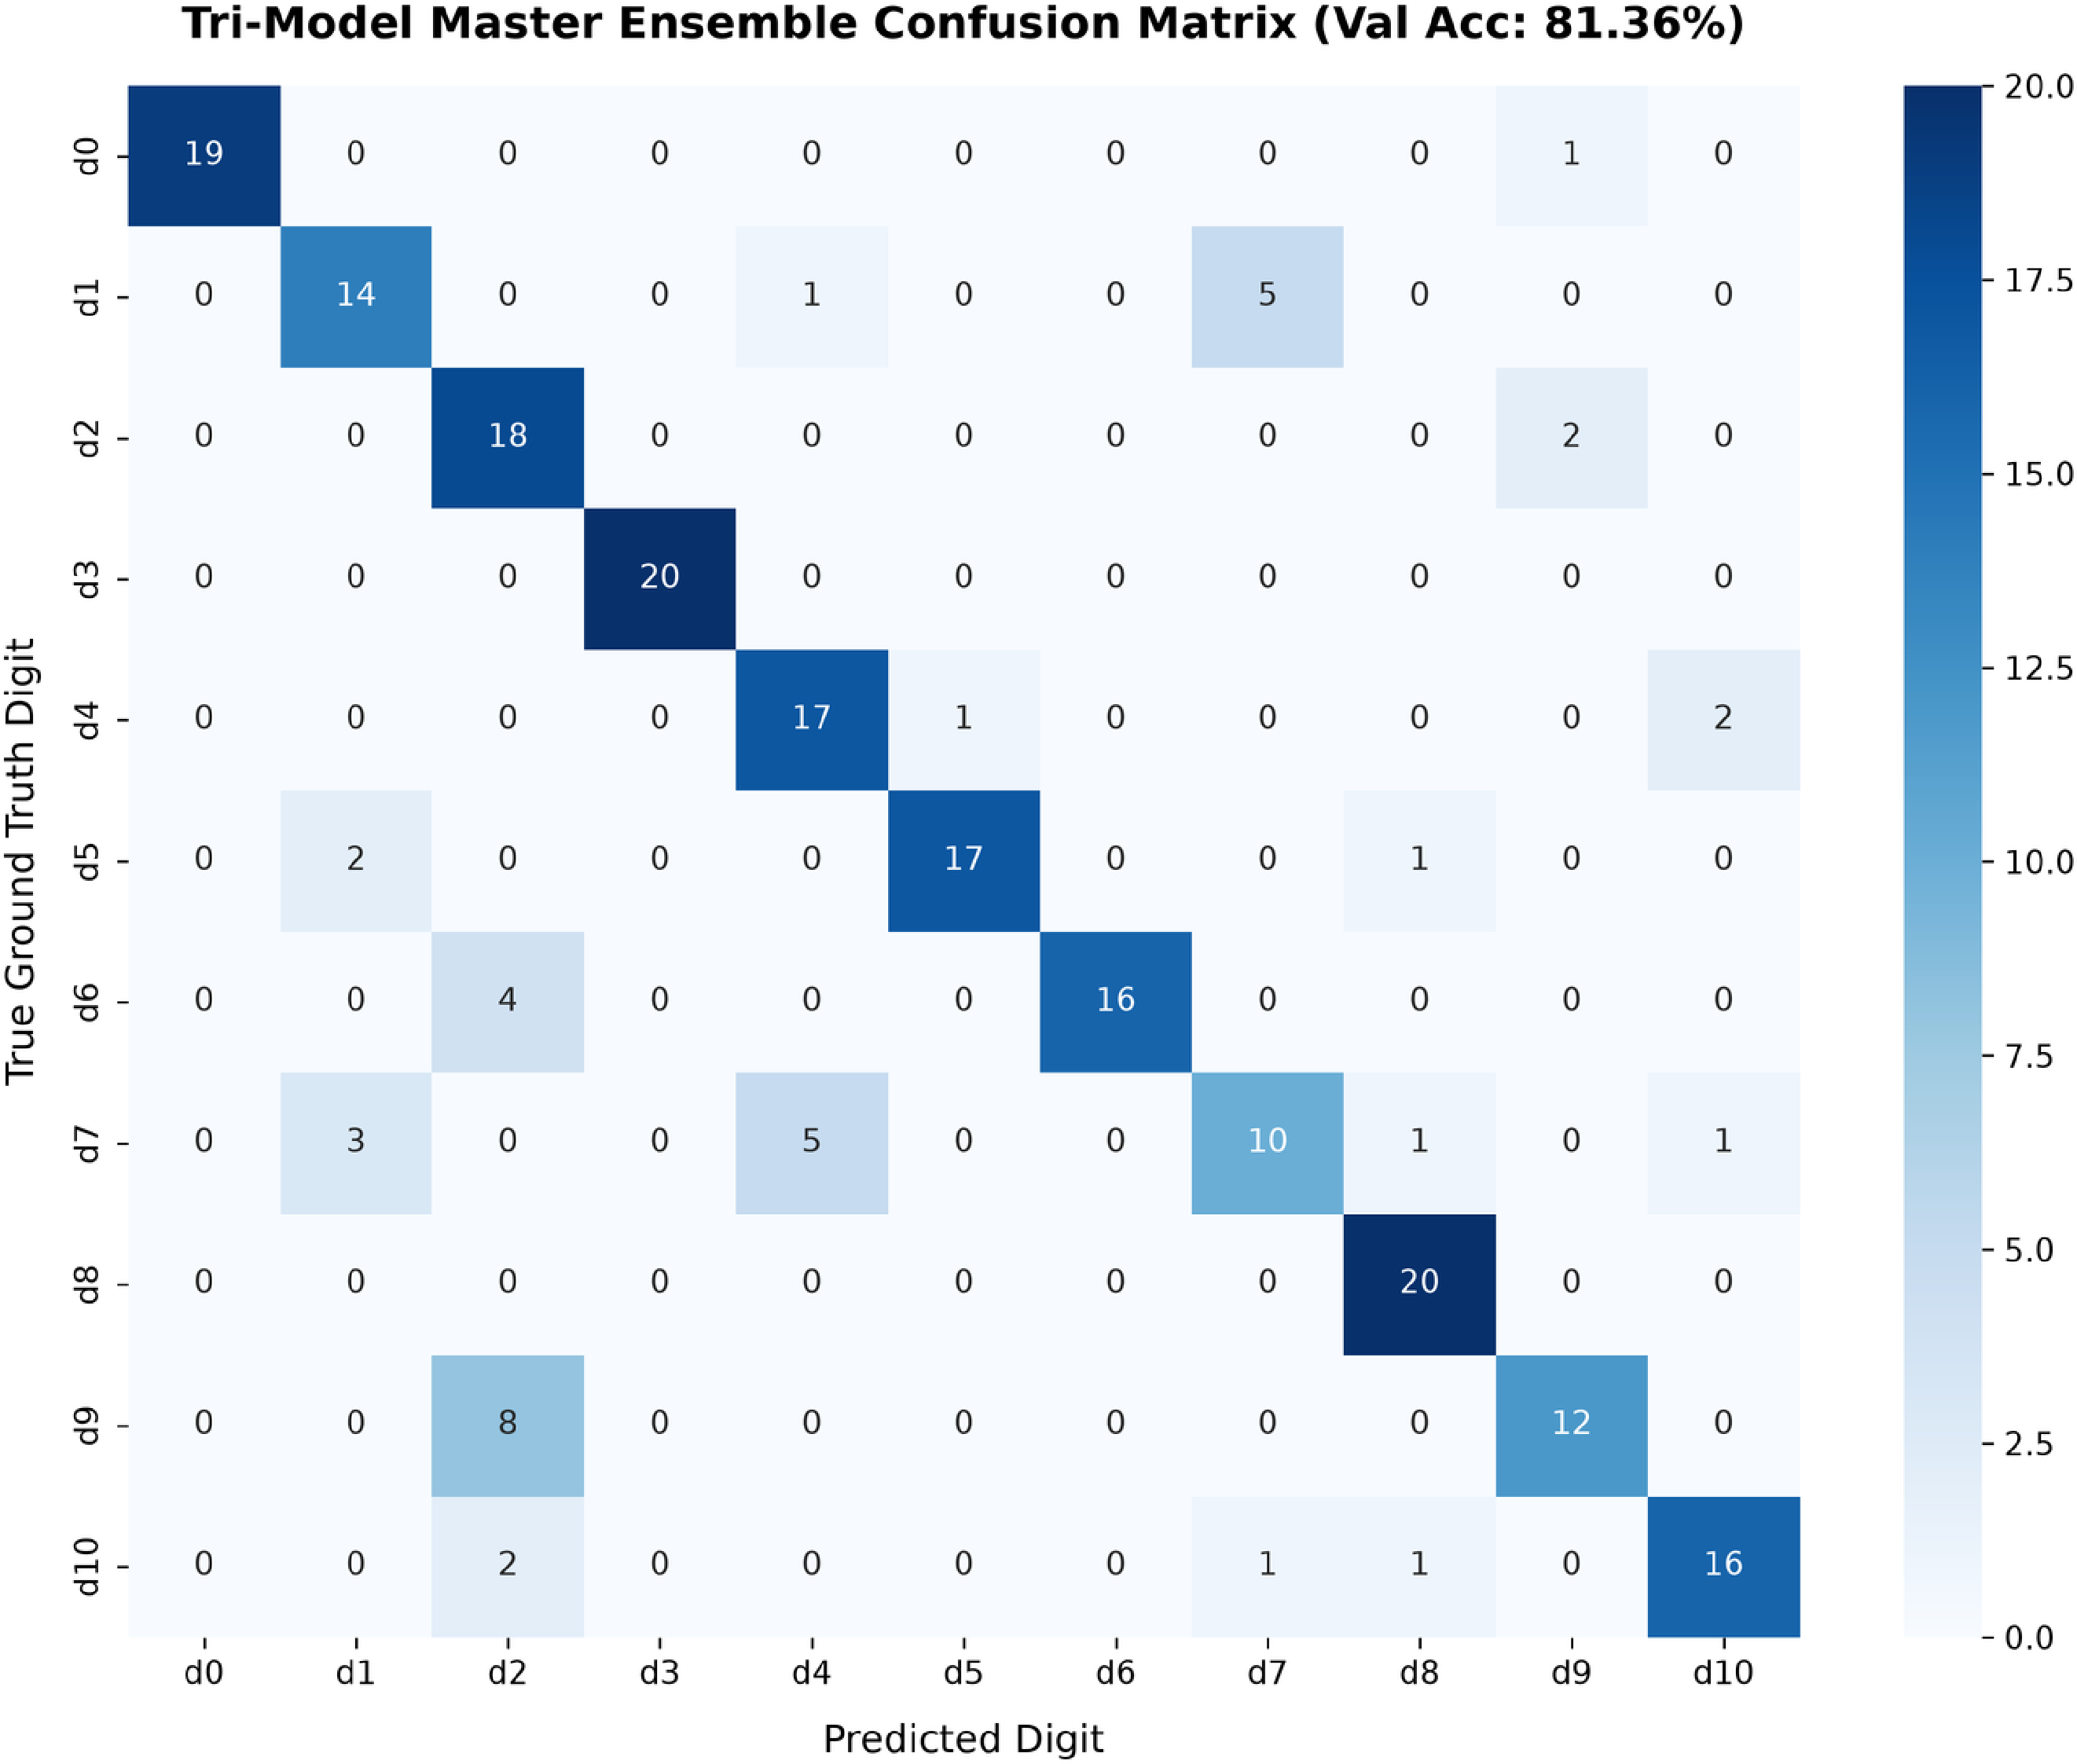
\includegraphics[width=0.96\linewidth]{figures/cm_tri.png}
    \end{center}
\end{columns}
\end{frame}

% ------------------------------------------------------------------------------
% Slide 12: Error analysis and Targeted Improvements
% ------------------------------------------------------------------------------
\begin{frame}
\frametitle{Error analysis and Targeted Improvements}

\vspace{-0.2cm}
\begin{columns}[onlytextwidth, T]
  \column{0.32\textwidth}
    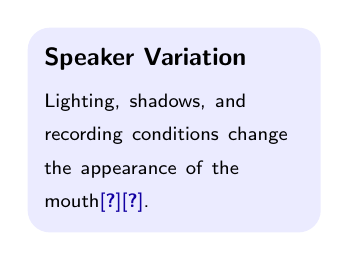
\begin{tikzpicture}
      \node[draw=none, fill=blue!8, rounded corners=8pt, text width=3.3cm, inner sep=6pt, minimum height=2.6cm] {
        {\fontsize{9.5}{12}\selectfont\textbf{Speaker Variation}}\\[0.12cm]
        {\fontsize{7.5}{10}\selectfont
        Lighting, shadows, and recording conditions change the appearance of the mouth\cite{lyngdoh2026}\cite{prajwal2022}.}
      };
    \end{tikzpicture}

  \column{0.32\textwidth}
    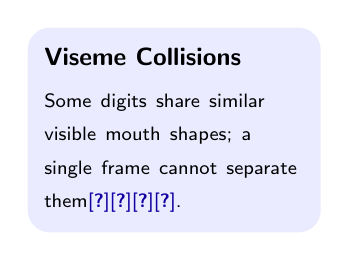
\begin{tikzpicture}
      \node[draw=none, fill=blue!8, rounded corners=8pt, text width=3.3cm, inner sep=6pt, minimum height=2.6cm] {
        {\fontsize{9.5}{12}\selectfont\textbf{Viseme Collisions}}\\[0.12cm]
        {\fontsize{7.5}{10}\selectfont
        Some digits share similar visible mouth shapes; a single frame cannot separate them\cite{lyngdoh2026}\cite{prajwal2022}\cite{chung2017}\cite{thomas2025}.}
      };
    \end{tikzpicture}

  \column{0.32\textwidth}
    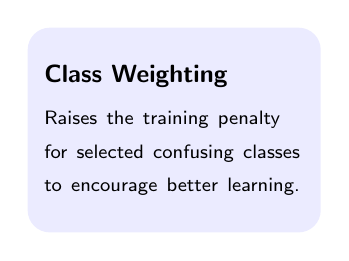
\begin{tikzpicture}
      \node[draw=none, fill=blue!8, rounded corners=8pt, text width=3.3cm, inner sep=6pt, minimum height=2.6cm] {
        {\fontsize{9.5}{12}\selectfont\textbf{Class Weighting}}\\[0.12cm]
        {\fontsize{7.5}{10}\selectfont
        Raises the training penalty for selected confusing classes to encourage better learning.}
      };
    \end{tikzpicture}
\end{columns}

\vspace{0.4cm}
{\fontsize{11}{14}\selectfont\textbf{Additional experiments}}\\[0.12cm]
{\fontsize{8.5}{12}\selectfont
\begin{itemize}
  \item \textbf{Test-time Augmentation (TTA):} average predictions from original, shifted, and flipped views\cite{prajwal2022}.
  \item \textbf{Motion channel:} add frame differences to highlight changing mouth regions
  \item \textbf{Focal Loss:} focus training more on hard-to-classify examples.
\end{itemize}}
\end{frame}

% ------------------------------------------------------------------------------
% Slide 13: Conclusion, Limitations and Next Steps
% ------------------------------------------------------------------------------
\begin{frame}
\frametitle{Conclusion, Limitations and Next Steps}

\vspace{-0.25cm}
\begin{columns}[onlytextwidth, T]
  \column{0.31\textwidth}
    {\fontsize{11}{14}\selectfont\textbf{\color{themeblue}Conclusion}}\\[0.15cm]
    {\fontsize{8}{11.5}\selectfont
    \begin{itemize}
      \item Transfer learning outperformed scratch training.
      \item Temporal modelling and attention helped.
      \item Diverse models improved results when combined.
    \end{itemize}}

  \column{0.32\textwidth}
    \hspace{-0.15cm}\vline\hspace{0.15cm}
    \begin{minipage}{0.92\linewidth}
    {\fontsize{11}{14}\selectfont\textbf{\color{themeblue}Limitations}}\\[0.15cm]
    {\fontsize{8}{11.5}\selectfont
    \begin{itemize}
      \item Small set of validation speakers\cite{lyngdoh2026}.
      \item Ensemble choices/weights selected using validation results.
      \item No independent held out test result is established here.
    \end{itemize}}
    \end{minipage}

  \column{0.33\textwidth}
    \hspace{-0.15cm}\vline\hspace{0.15cm}
    \begin{minipage}{0.92\linewidth}
    {\fontsize{11}{14}\selectfont\textbf{\color{themeblue}Next Steps}}\\[0.15cm]
    {\fontsize{8}{11.5}\selectfont
    \begin{itemize}
      \item Evaluate on completely held out speakers
      \item Use speaker level cross validation\cite{lyngdoh2026}.
      \item Improve difficult classes and reduce inference cost
    \end{itemize}}
    \end{minipage}
\end{columns}

\vspace{0.45cm}
{\fontsize{10}{13}\selectfont\textbf{\color{themeblue}Main conclusion}}\\[0.1cm]
{\fontsize{8.5}{12}\selectfont
The three-model ensemble reached \textbf{81.36\%} on the reported validation set by combining spatial features, mouth-motion cues and different temporal attention strategies. Independent evaluation is needed to confirm generalization.}
\end{frame}

% ------------------------------------------------------------------------------
% Slide 14: References I
% ------------------------------------------------------------------------------
\begin{frame}
\frametitle{References I}

\vspace{-0.2cm}
\begin{thebibliography}{9}
  \bibitem{prasad2025}
  R.~K. Prasad, D.~Kalita, Z.~M. Mondal, M.~T. Singh, S.~M.~S. Askari, and C.~Kalita,
  ``Analysis of Lip Reading of Assamese Digits using Deep Learning,''
  \textit{Science \& Technology Journal}, vol.~13, no.~1, 2025.
  \href{https://doi.org/10.22232/stj.2025.13.01}{\underline{Read paper}}

  \vspace{0.2cm}
  \bibitem{lyngdoh2026}
  E.~L. Lyngdoh and A.~Maji,
  ``Lip Reading in Khasi Language using few Machine Learning Techniques,''
  \textit{Procedia Computer Science}, vol.~283, pp.~3493--3503, 2026.
  \href{https://doi.org/10.1016/j.procs.2026.01.001}{\underline{Read paper.}}

  \vspace{0.2cm}
  \bibitem{kim2023}
  M.~Kim, J.~H. Yeo, J.~Choi, and Y.~M. Ro,
  ``Lip Reading for Low-Resource Languages by Learning and Combining General Speech Knowledge and Language-Specific Knowledge,''
  in \textit{Proceedings of ICCV}, pp.~15359--15371, 2023.
  \href{https://openaccess.thecvf.com/content/ICCV2023/html/Kim_Lip_Reading_for_Low-Resource_Languages_by_Learning_and_Combining_General_ICCV_2023_paper.html}{\underline{Read paper.}}

  \vspace{0.2cm}
  \bibitem{yeo2023}
  J.~H. Yeo, M.~Kim, S.~Watanabe, and Y.~M. Ro,
  ``Visual Speech Recognition for Languages with Limited Labeled Data using Automatic Labels from Whisper,''
  \textit{arXiv preprint arXiv:2309.08535}, 2023.
  \href{https://arxiv.org/abs/2309.08535}{\underline{Read paper.}}
\end{thebibliography}
\end{frame}

% ------------------------------------------------------------------------------
% Slide 15: References II
% ------------------------------------------------------------------------------
\begin{frame}
\frametitle{References II}

\vspace{-0.25cm}
{\fontsize{8}{10.5}\selectfont
\begin{thebibliography}{9}
  \setcounter{enumiv}{4}

  \bibitem{prajwal2022}
  K.~R. Prajwal, T.~Afouras, and A.~Zisserman,
  ``Sub-Word Level Lip Reading With Visual Attention,''
  in \textit{Proceedings of CVPR}, pp.~5162--5172, 2022.
  \href{https://arxiv.org/abs/2203.02447}{\underline{Read paper.}}

  \vspace{0.08cm}
  \bibitem{chung2017}
  J.~S. Chung and A.~Zisserman,
  ``Lip Reading in the Wild,''
  in \textit{Computer Vision -- ACCV 2016, Lecture Notes in Computer Science}, vol.~10112, pp.~87--103, 2017.
  \href{https://www.robots.ox.ac.uk/~vgg/publications/2016/Chung16a/}{\underline{Read paper.}}

  \vspace{0.08cm}
  \bibitem{rahmatullah2025}
  G.~M. Rahmatullah, S.-J. Ruan, and L.~P.-H. Li,
  ``Visual Speech Recognition Using Attention-Enhanced ResNet and Hybrid Recurrent-Transformer Encoder with Quantity-Ratio Curriculum Learning for Low-Resource Languages,''
  \textit{Neurocomputing}, vol.~654, article 131303, 2025.
  \href{https://doi.org/10.1016/j.neucom.2025.131303}{\underline{Read paper.}}

  \vspace{0.08cm}
  \bibitem{thomas2025}
  M.~Thomas, E.~Fish, and R.~Bowden,
  ``VALLR: Visual ASR Language Model for Lip Reading,''
  in \textit{Proceedings of ICCV}, pp.~2846--2856, 2025.
  \href{https://openaccess.thecvf.com/content/ICCV2025/html/Thomas_VALLR_Visual_ASR_Language_Model_for_Lip_Reading_ICCV_2025_paper.html}{\underline{Read paper.}}

  \vspace{0.08cm}
  \bibitem{deka2025}
  J.~R. Deka and M.~Phil,
  ``Studying the Adjectives of Tai-Phake, an Endangered Language of Assam,''
  \textit{Strength for Today and Bright Hope for Tomorrow}, vol.~25, no.~4, p.~197, 2025.
  \href{http://www.languageinindia.com/}{\underline{Read paper.}}
\end{thebibliography}}
\end{frame}

% ------------------------------------------------------------------------------
% Slide 16: Thank you
% ------------------------------------------------------------------------------
\begin{frame}
\begin{center}
  \vspace{2.5cm}
  {\fontsize{36}{42}\selectfont\textbf{THANK YOU!}}
\end{center}
\end{frame}

\end{document}
